\section{Interferometry and the Inverse Problem}\label{intro}
Radio Antennas in Astronomy require a sub-arcsecond angular resolution. For a single dish antenna, the angular resolution is $ \theta \approx \lambda / D$ radians, which leads to impossibly large diameters for radio wavelengths. Interferometers, where several dishes act as a single instrument, can achieve a high angular resolution for an economical price.  (Radio Astronomy has a lot of interest in Interferometers, building VLA, ALMA, LOFAR and planning SKA). However Interferometers do not observe the sky directly. Each antenna pair measures a Fourier component of the observed image. Furthermore the Fourier space is not fully samnpled, it is incomplete. The task is to reconstruct an image in Pixel space from an incomplete set of Fourier measurements (Visibilities). From here on forward term Visibility is used. It is interchangeable with Fourier Component.

Each antenna pair, quadratic number of data points with the number of antennas: a lot of data)(An interferometer does not observe the image directly. Simplified, each antenna pair observes a Fourier component of the An Antenna Pair measures a fourier component of the image.) (If all the fourier components are measured, the observed image could be retrieved by calculating the inverse fourier transform. However, only a limited set of visibilites can be measured.)(Inverting the problem results in an image with artefacts (Dirty Image).) (Clean can solve it for the current class of interferometers)

%(Future Interferometers like the Square Kilometer Array do introduce additional problems in the inverse Problem.)(Modelling the new effects)(while being able to handle the large amount of data.)

% The Inverse Problem. Radio Astronomy has come up with the CLEAN class Algorithms that work well in practice for current radio interferometers.
%The theory of Compressed Sensing \cite{candes2006robust} \cite{donoho2006compressed}


\subsection{Simplified Inverse Problem}
For the current class of interferometers, retrieving the observed image of the sky is calculating the Inverse Fourier Transform of the measured Visibilities. (This is a simplification of the actual problem, which does not hold true for future instruments like SKA. How the Inverse Problem changes for future instruments is handled in section \ref{radio}). Since the Visibility Space is undersampled, the resulting image is 'dirty', as it contains effects from the instrument. The effects of the instrument can be modelled as a Point Spread Function (PSF). The Dirty Image is the Result of the True Image convolved with the PSF. Figure \ref{intro:inverse_problem} shows an example of the PSF, Dirty Image and True Image.
\begin{figure}[h!]
	\centering
	\begin{subfigure}[b]{0.3\linewidth}
		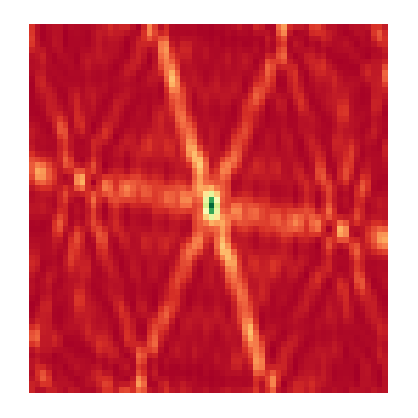
\includegraphics[width=\linewidth, trim={18px 19px 18px 18px}, clip]{./chapters/01.intro/img/psf.png}
		\caption{Point Spread Function (PSF)}
	\end{subfigure}
	\begin{subfigure}[b]{0.3\linewidth}
		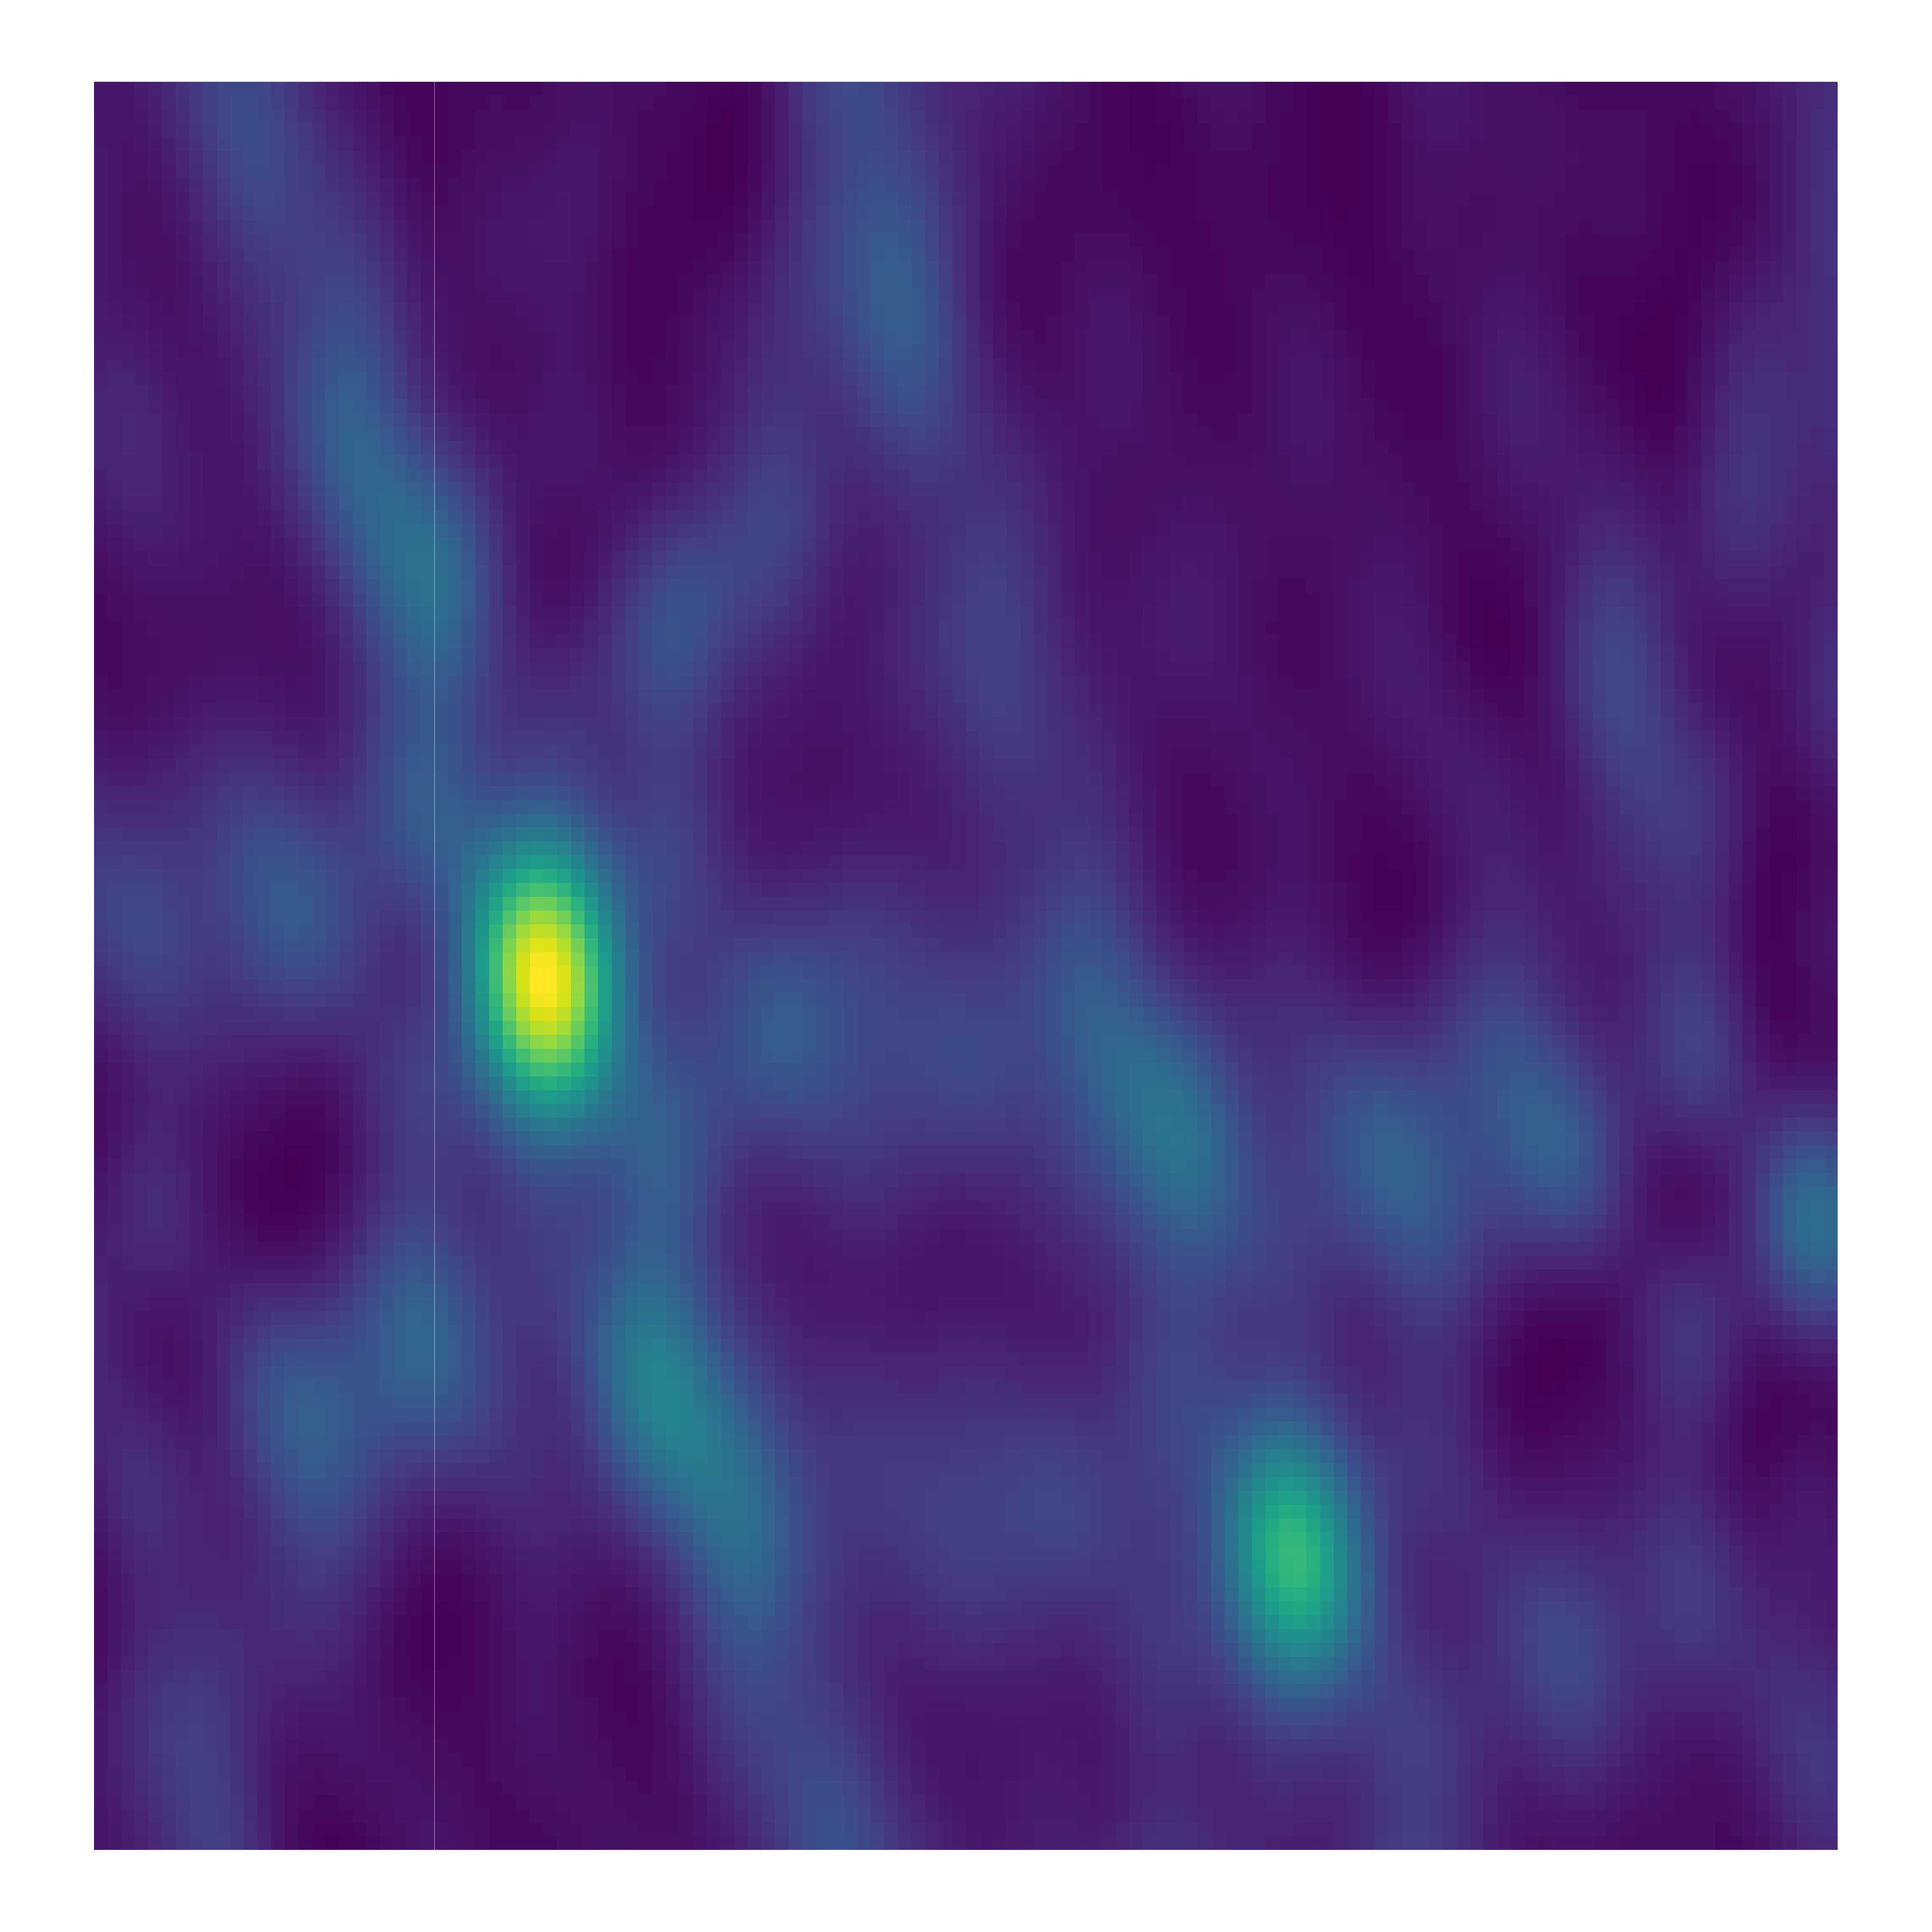
\includegraphics[width=\linewidth, trim={18px 19px 18px 18px}, clip]{./chapters/01.intro/img/dirty_image.png}
		\caption{Dirty Image}
	\end{subfigure}
	\begin{subfigure}[b]{0.3\linewidth}
		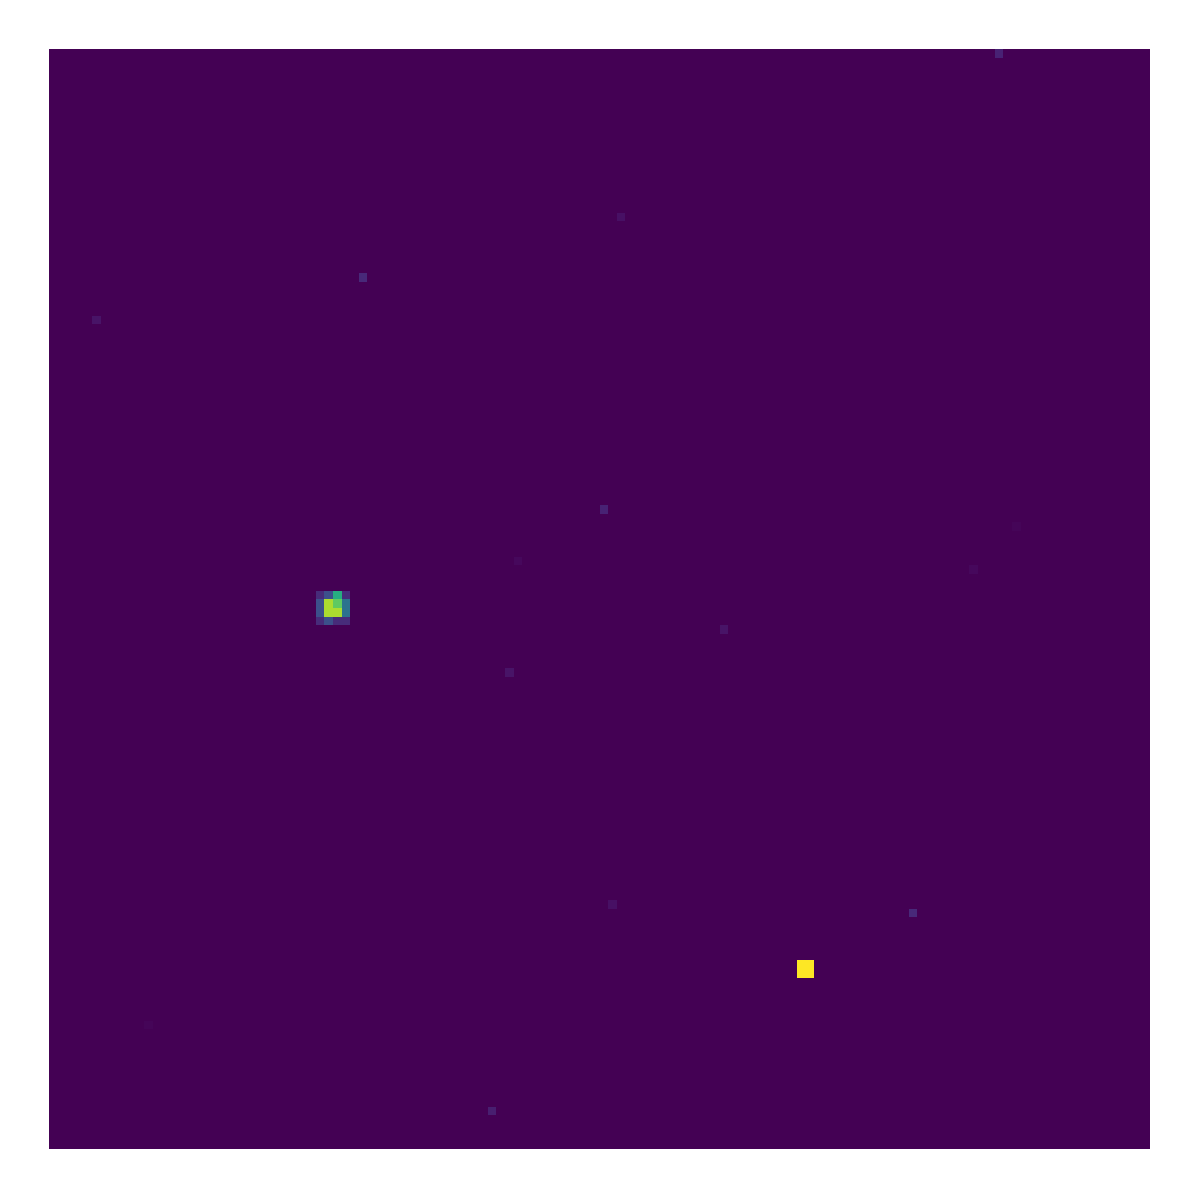
\includegraphics[width=\linewidth, trim={18px 19px 18px 18px}, clip]{./chapters/01.intro/img/true_image.png}
		\caption{True Image}
	\end{subfigure}
	\caption{The Inverse Problem: Finding the true image of the sky when only the PSF and the dirty image are known.}
	\label{intro:inverse_problem}
\end{figure}

The Dirty Image is the result of the Inverse Fourier Transform, the PSF on the other hand follows directly from the antenna configuration. Figure \ref{intro:ANT_UV_PSF} shows an example of the VLA instrument. 

\begin{figure}[h!]
	\centering
	\begin{subfigure}[b]{0.3\linewidth}
		 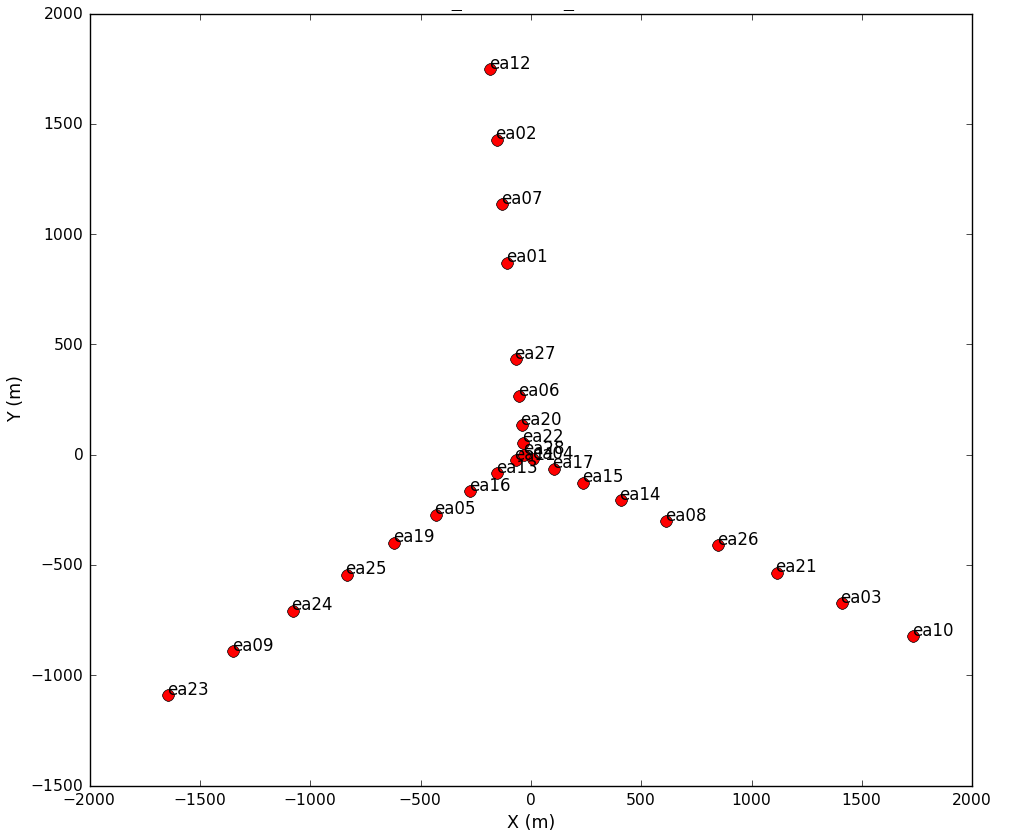
\includegraphics[width=\linewidth, trim={18px 19px 18px 18px}, clip]{./chapters/01.intro/img/antennas.png}
		 \caption{Antenna Configuration}
	\end{subfigure}
	\begin{subfigure}[b]{0.3\linewidth}
		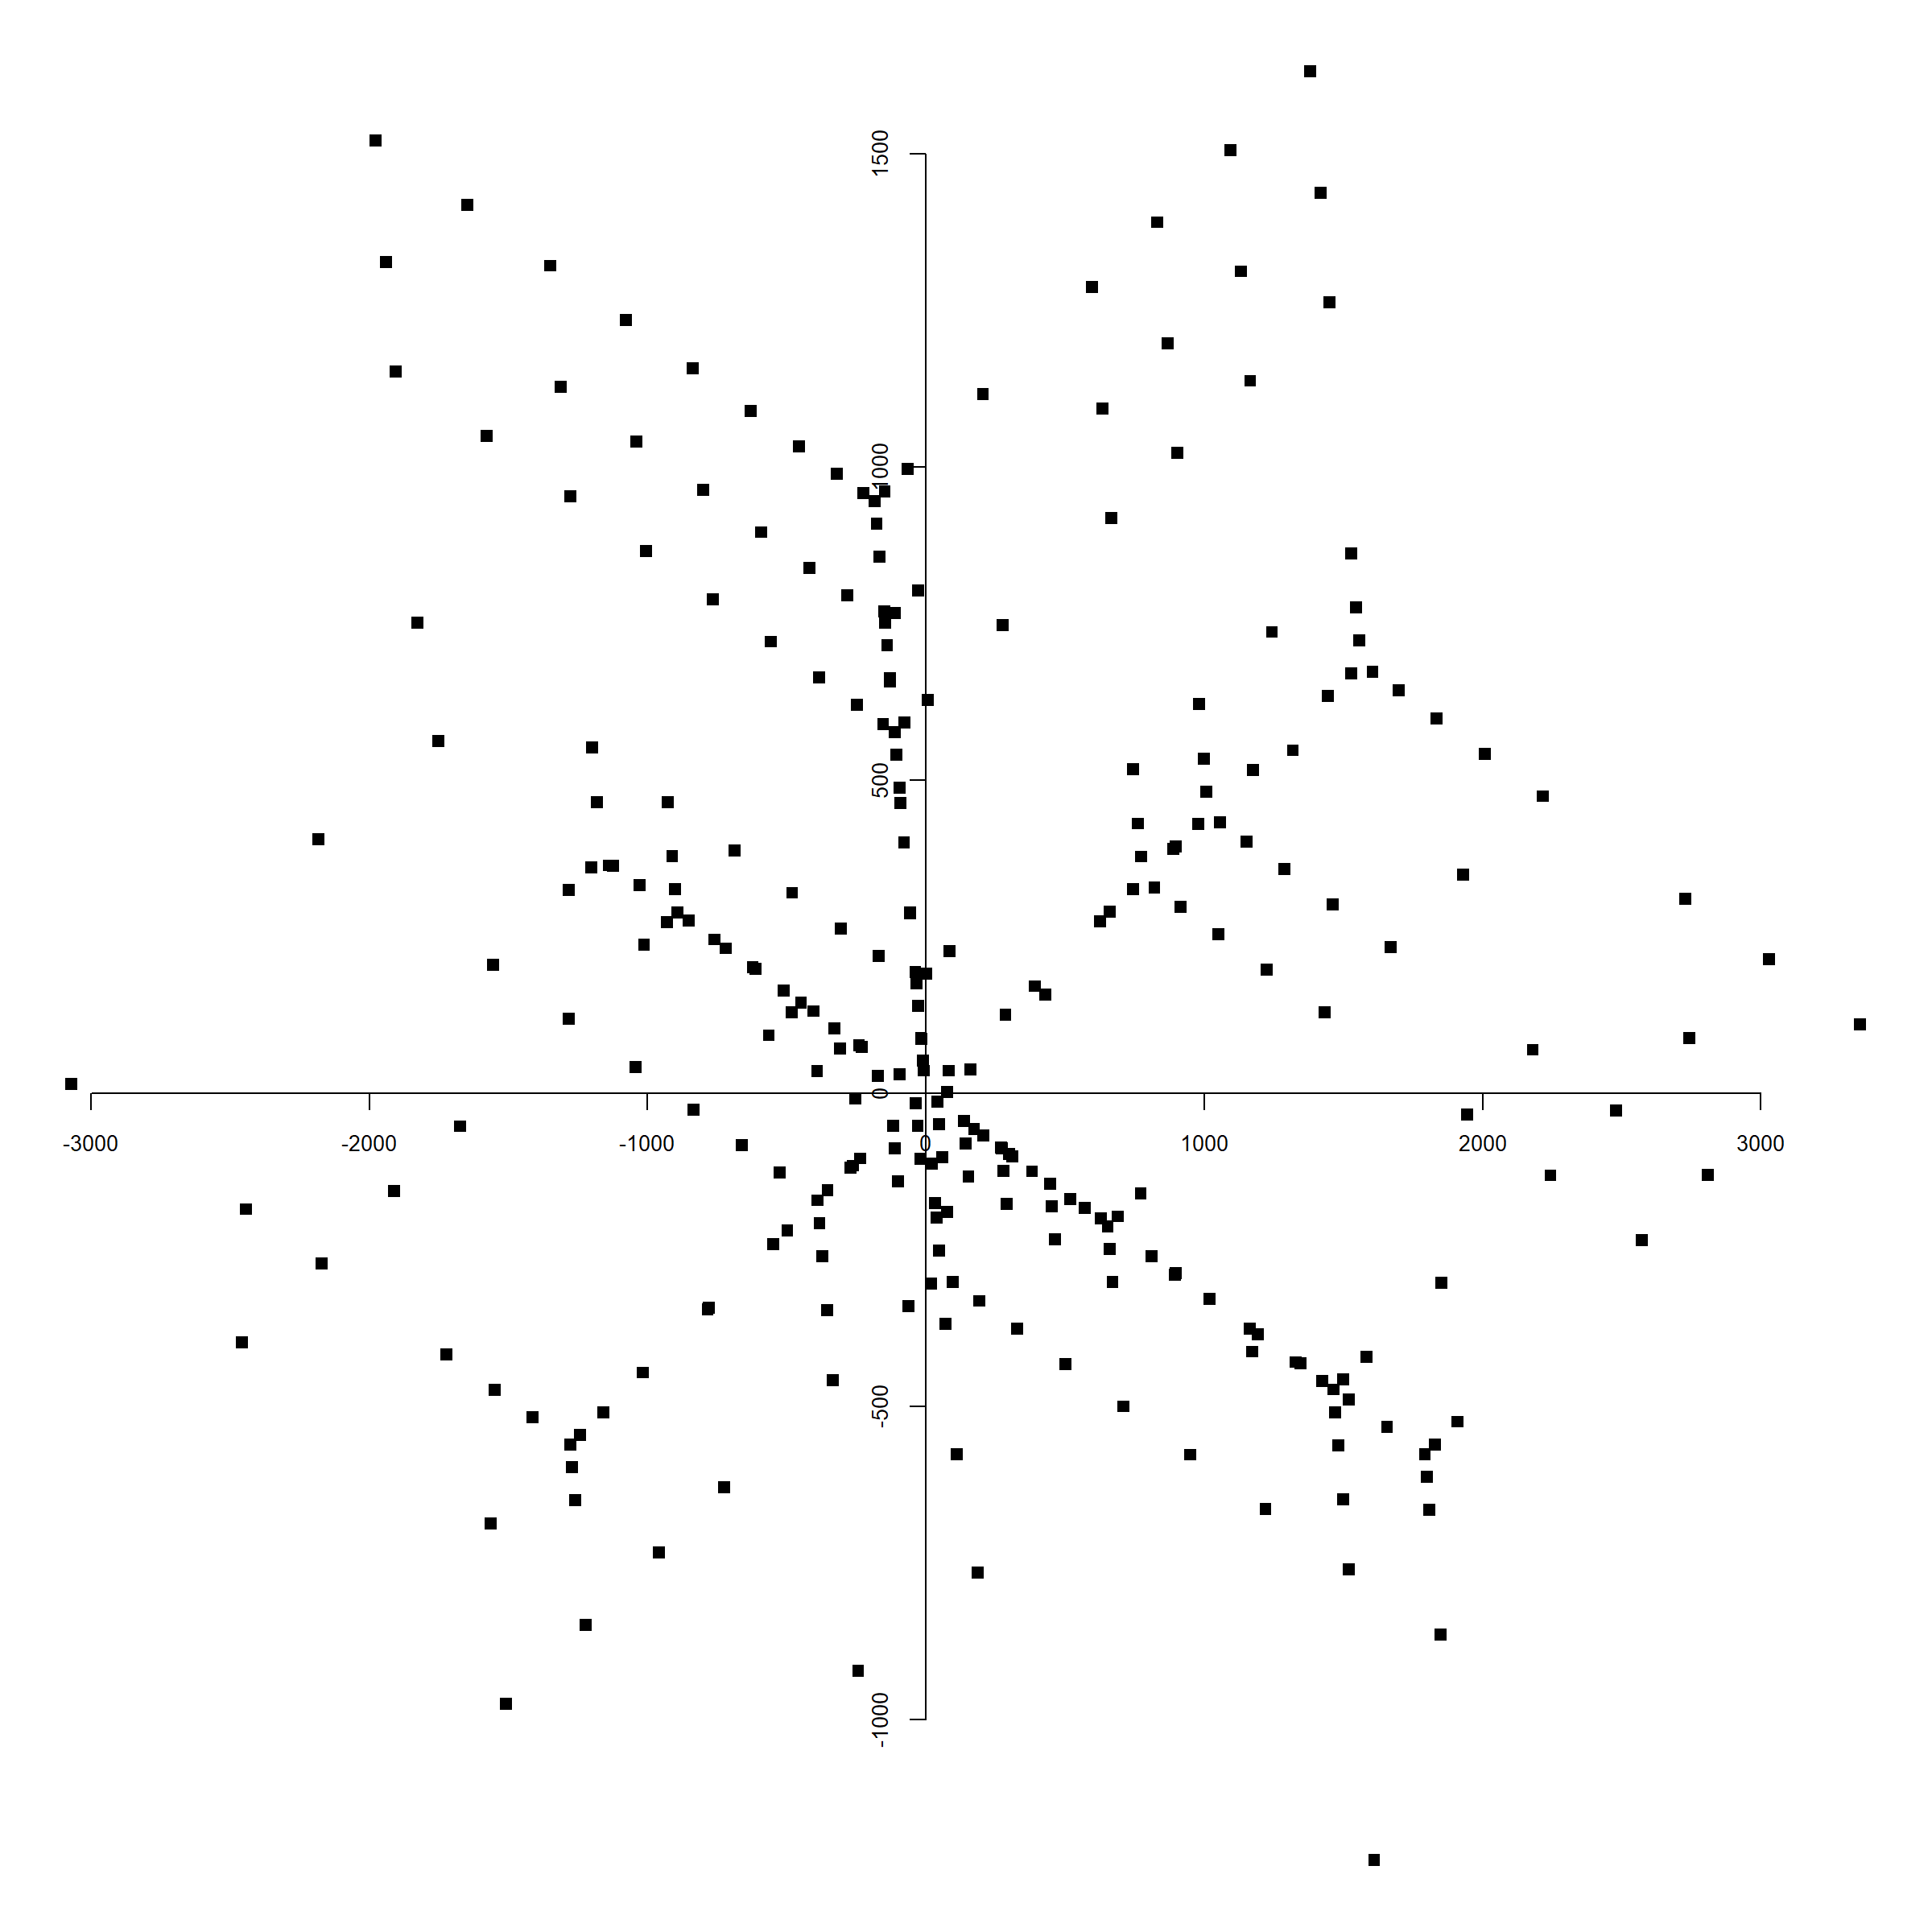
\includegraphics[width=\linewidth, trim={18px 19px 18px 18px}, clip]{./chapters/01.intro/img/uv.png}
		\caption{UV Space}
	\end{subfigure}
	\begin{subfigure}[b]{0.3\linewidth}
		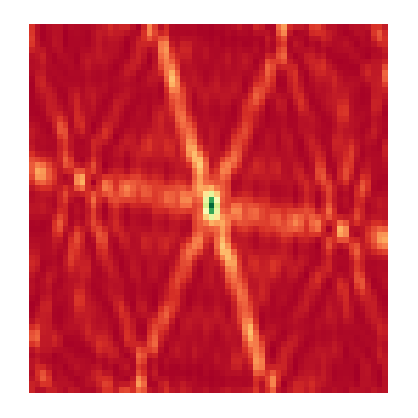
\includegraphics[width=\linewidth, trim={18px 19px 18px 18px}, clip]{./chapters/01.intro/img/psf.png}
		\caption{Point Spread Function (PSF)}
	\end{subfigure}
	\caption{The Antenna Configuration sets up the UV Space. The UV Space dictates the PSF.}
	\label{intro:ANT_UV_PSF}
\end{figure}

Each antenna pair samples a point in the UV Space. The distance between the antenna pair is called the baseline. Shorter baselines sample UV-Points closer to the center, while longer baselines sample points further away.  Each point in the UV Space represents a frequency Visibilities of the observed image: High frequency components are located away from the center and low frequency components are towards the center. Since each antenna pair contributes a Visibility, an Interferometer of $N$ antennas measures $(N-1)/2$ Visibilities. The configuration of the antenna sets up which points are sampled in the UV Space. The PSF can be calculated by using the Inverse Fourier Transform on the UV-Space.

Since the Dirty Image and the PSF are known, one needs to deconvolve the Dirty Image with the PSF and try to retrieve the True Image. More formally, it tries to find $X$ from the equation \eqref{intro:eq:deconvolve} in a noiseless environment.

\begin{equation}\label{intro:eq:deconvolve}
X \star  PSF = D_{dirty} 
\end{equation}


\subsection{Deconvolution with CLEAN}
The CLEAN class of Algorithms\cite{hogbom1974aperture}\cite{schwab1984relaxing}\cite{rich2008multi}\cite{rau2011multi} are widely used in Radio Astronomy. It does not solve the deconvolution problem \eqref{intro:eq:deconvolve} directly. Instead, it minimizes a similar optimization problem with the objective  \eqref{intro:eq:clean}. In each iteration, CLEAN searches the highest peak in $D_{dirty}$ and removes a fraction of the PSF at that point. It is a greedy optimizes the objective \eqref{intro:eq:clean}. It is easy to show that if CLEAN minimizes the objective to zero, then it has found a solution to the original problem \eqref{intro:eq:deconvolve}. 

\begin{equation}\label{intro:eq:clean}
\underset{X}{minimize} \: \left \| D_{dirty} - X \star PSF \right \|_2^2
\end{equation}

In a noiseless environment, the true image would be located where the objective of \eqref{intro:eq:clean} is zero. In the real world however, noise corrupts the problem and the true image may not be at the minimum any more. To address this, CLEAN is stopped early by limiting the number of iterations or when the peak is below a threshold. The algorithm should find the minimum of the objective \eqref{intro:eq:clean} where only a limited number of pixels are allowed to be non-zero; an implicit regularization term. With the right parameters, the regularization should stop the noise from corrupting the result and CLEAN should reproduce the true image.

So does CLEAN reproduce the image? It can, but it does not have to. The algorithm has no guarantees, we do not even know if the result is close to the true image. 


\subsection{From CLEAN to Compressed Sensing}
CLEAN can be converted into the Compressed Sensing Framework. First, the regularization term has to be explicit, it gets added to the objective function. The resulting objective \eqref{intro:eq:csclean} has two terms: A data term and a regularization term. The data term forces the reconstruction to be close to the measurement, while the regularization term forces the reconstruction to be plausible. $\lambda$ models the tradeoff between the terms. Note that the zero norm $\left \| PX \right \|_0$ acts as an indicator function and is not technically a norm.

\begin{equation}\label{intro:eq:csclean}
\underset{X}{minimize} \: \left \| D_{dirty} -X \star PSF \right \|_2^2 \: + \: \lambda \left \| PX \right \|_0
\end{equation}

When $P$ is the identity matrix, the new objective is the Compressed Sensing version of CLEAN. It assumes that the reconstruction is sparse in the image domain. This is true when there are only a few point sources located in the image. Extended sources are are not well represented and are harder to detect. The objective function is optimized by a greedy solver. An Algorithm in the Compressed Sensing Framework needs three parts:
\begin{itemize}
	\item An objective function with a data and regularization term
	\item A Matrix $P$ in which the signal can be sparsely represented.
	\item An optimization algorithm that is able to handle the objective function
\end{itemize}

The important questions are: In an undersampled, noisy environment, does the new objective \eqref{intro:eq:csclean} have a global minimum? What is the chances that the minimum is equal to the true image? It turns out that even though we have fewer samples than the Nyquist-Shannon Theorem requires, we can guarantee a global minimum and that the minimum is equal to the true image, if we have enough prior knowledge $P$ about the signal. How we model the signal and by extend, what $P$ we choose is essential for Compressed Sensing

\subsubsection{Modelling Prior Knowledge and Compressible Signals}
The objective \eqref{intro:eq:csclean} requires the product $PX$ to be sparse (produces few non-zero entries) when $X$ is plausible. This the same requirement as a compression algorithm and indeed, if we know our signal is compressible in the wavelet domain, then the wavelet transform is a good $P$ for Compressed Sensing. But $P$ is not limited to a transformation. The only requirement is that the signal's representation is as sparse as possible. There is a case for overcomplete representations for compressed sensing (vis-cs). 

$P$ should be incoherent from the measurements

How sparsely the signal can be represented dictates how many samples are needed Restricted Isometry Property, RIP 

